% Please use the skeleton file you have received in the
% invitation-to-submit email, where your data are already
% filled in. Otherwise please make sure you insert your
% data according to the instructions in PoSauthmanual.pdf
\documentclass{PoS}
\usepackage{bm}
\usepackage{csquotes}
\usepackage{amsmath}

\title{$\bm{b}$-flavour tagging in $\bm{p\!p}$ collisions}

\ShortTitle{Flavour Tagging at LHCb}

\author{\speaker{Alex Birnkraut}\\%\thanks{A footnote may follow.}\\
        TU Dortmund\\
        E-mail: \email{a.birnkraut@cern.ch}}

%\author{Another Author\\
%        Affiliation\\
%        E-mail: \email{...}}

\abstract{In the system of neutral $B^0$ mesons $C\!P$-violating processes can be measured using time dependent analyses, as performed at the LHCb experiment. For such analyses the knowledge of the initial flavour of the mesons is mandatory. This information is provided by the Flavour Tagging, which exploits a variety of different algorithms. This article shows the good performance in different analyses which allowed high precision measurements and also the improvements which were made throughout Run I. Finally some very recent developments and new algorithms to tag the initial flavour are described.}

\FullConference{The European Physical Society Conference on High Energy Physics\\
		22--29 July 2015\\
		Vienna, Austria}


\begin{document}

\section{Introduction}\label{sec:1}

The aim of the Flavour Tagging algorithms is to determine the initial flavour of the signal $B$ meson. These algorithms are called taggers and can be classified in two groups. The so called same side (SS) taggers use charged particles which are created in the fragmentation process of the $b$ quark of the signal $B$ meson. The opposite side (OS) taggers exploit the flavour if the non-signal $b$ quark of the initial $b\bar{b}$ pair and use then the correlation at between the two flavours at production.\\
In this article in section \ref{sec:2} the algorithms used at LHCb are dsecribed more in detail and the characteristics of the performance of the Flavour Tagging are presented. The calibration of the Flavour Tagging is then explained in section \ref{sec:3}, in section \ref{sec:4} physics analyses at LHCb from the LHC Run I are presented and the improvements which were made are shown. Last, before giving a short conclusion in section \ref{sec:6} some recent developments of new flavour tagging algorithms are illustrated in section \ref{sec:5}. 

\section{Flavour Tagging algorithms at LHCb}\label{sec:2}

To measure time dependent flavour oscillations or $C/!P$ asymmetries  in neutral $B$ meson systems the knowledge of the $b$ quark flavour at production is mandatory. To retain this information two different classes of algorithms are used at LHCb. As explained in section \ref{sec:1} these classes are the opposite and same side taggers (Figure \ref{fig:flavtagscheme}).
\begin{figure}[htbp]
	\begin{center}
		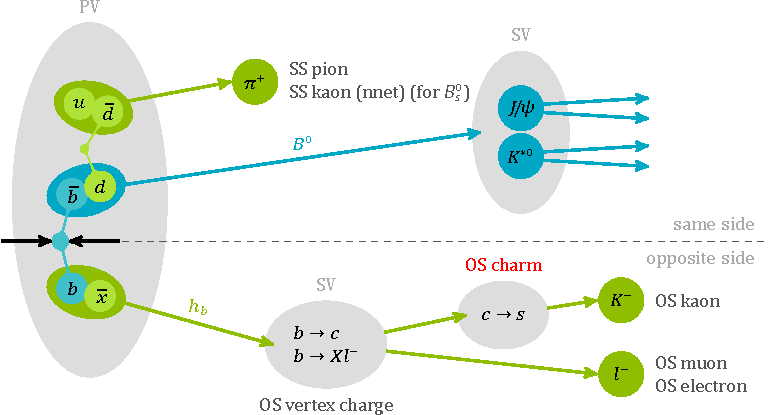
\includegraphics[width=0.8\textwidth, angle=0]{figs/FlavourTaggerScheme.pdf}
		\caption{Scheme of the different flavour tagging algorithms. Same side taggers are shown in the upper part, opposite side taggers in the lower part.}
		\label{fig:flavtagscheme}
	\end{center}
\end{figure}
Each tagger then provides a decision $d$ on the initial flavour (\enquote{tag}) and a probability $\eta$ to be wrong.

\subsection{Opposite side tagging}

The tagging information in the opposite side are obtained with mainly four different types of algoroithms. The two lepton taggers, the OS electron and the OS muon tagger, use semileptonic decays of the opposite $b$ quark. If the initial $b$ hadron has not mixed the charge of the lepton indicates then indicates the initial flavour of the $b$ quark. The OS kaon and the OS charm taggers use quite similar approaches by analysing the decay product of the decay chain $b\to c\to s$ or the decay product of the decay chain $b\to c$, respectively. The charge of the final state kaon in case of the OS kaon or the $D$ meson in case of the OS charm tagger are used to get information about the initial $b$ flavour. \\
In contrast to this method the OS vertex charge tagger does not use single tracks but a weighted charge of the whole secondary vertex to come to a tag decision. In order to do so, the secondary vertex is reconstructed first out of two tracks which have the highest probablity to originate from the $b$ hadron. After this, more tracks are added to the vertex and the weighted charge is calculated as
\begin{equation}
Q_\text{vtx}=\frac{\sum_i p_T^k(i)Q_i}{\sum_i p_T^k(i)}
\end{equation}  
The opposite side tagging is independent of the signal $B$ meson as it only investigates the propagation of the opposite $b$ quark.

\subsection{Same side tagging}

For the same side tagging one has to distinguish between $B_d^0$ and $B_s^0$ mesons as the accompanying quark is a $d$ or a $s$ quark, respectively. In case of a $B_d^0$ meson an additional $d$ quark which can hadronise with an $u$ quark into a pion emerges. Also pions from excited states as $B^*$ and $B^**$ have the same charge as pions from the direct fragmenation process with a $B$ meson. If the signal $B$ meson is a $B_s^0$ an kaon can be formed out of the additional $s$ quark and an $u$ quark. In a new development the fragmentation kaon is selected using neural nets. The so called SS kaon neural net tagger will be described more in detail in section \ref{sec:5}.

\subsection{Flavour Tagging characteristics}

Each tagger provides for each candidate a tag $d$ and the probability $\eta$ that this tag is wrong. The tag can be $1$ for a $\bar{b}$ quark, $-1$ for a $b$ quark and $0$ if the tagger could not provide a tag decision. The mistag probability is defined to smaller then $0.5$ as the tag could be flipped otherwise. This mistag is just a self-estimation of the tagger and the true mistag is defined as
\begin{equation}
\omega=\frac{N_\text{wrong}}{N_\text{right}+N_\text{wrong}}
\end{equation}
where $N_\text{wrong}$ is the number of wrong tagged candidates and $N_\text{right}$ the number of correctly tagged candidates. Also the performance of the different taggers is described by their efficiencies
\begin{equation}
\varepsilon_\text{tag}=\frac{N_\text{right}+N_\text{wrong}}{N_\text{all}}
\end{equation}
with the number of wrong tagged ($N_\text{wrong}$) correctly tagged ($N_\text{right}$) and all ($N_\text{all}$) candidates and the effective tagging efficiency 
\begin{equation}
\varepsilon_\text{eff}=\varepsilon_\text{tag}\left(1-2\omega\right)^2.
\end{equation}
The effective tagging efficiency indicates the statistical degradation of the information and can thus be used to compare the performance of different tagging algorithms with each other and also in different decay modes.

\section{Calibration of the Flavour Tagging}\label{sec:3}

The mistag estimate $\eta$ provided by the different tagging algorithms has to be corrected and transformed into the true mistag probabilty $\omega$. This is done with a linear calibration function
\begin{equation}
\omega(\eta)=p_0+p_1\left(\eta-\langle\eta\rangle\right)\label{eq:linfunc}
\end{equation}
with the mean mistag estimate $\langle\eta\rangle$. The parameters $p_0$ and $p_1$ of this calibration function are extracted in to different ways. With charged decay modes as $B^+\to J\!/\!\psi K^+$ and $B^+\to D^0\pi^+$ the true mistag $\omega$ can be extracted by comparing the tag with the charge of the kaon or pion in the final state. In neutral decay modes as $B^0\to J\!/\!\psi K^{*0}$, $B^0\to D^{*-}\mu^+\nu_\mu$ or $B_s^0\to D_s^-\pi^+$ a full time-dependent analysis is necessary to extract omega from the mixing asymmetry:
\begin{equation}
A_\text{mix}(t)\propto\left(1-2\omega\right)\cos\left(\Delta m_{d/s} t\right)
\end{equation}
In both cases the calculation of $\omega$ is done in bins of the mistag estimate $\eta$ and the linear function \ref{eq:linfunc} is fitted to the $(\omega,\eta)$ pairs. Figure \ref{fig:calibration} shows for one bin the time dependent mixing asymmetry and the linear calibration function for the calibration mode $B^0\to J\!/\!\psi K^{*0}$. 
\begin{figure}[htbp]
	\begin{center}
		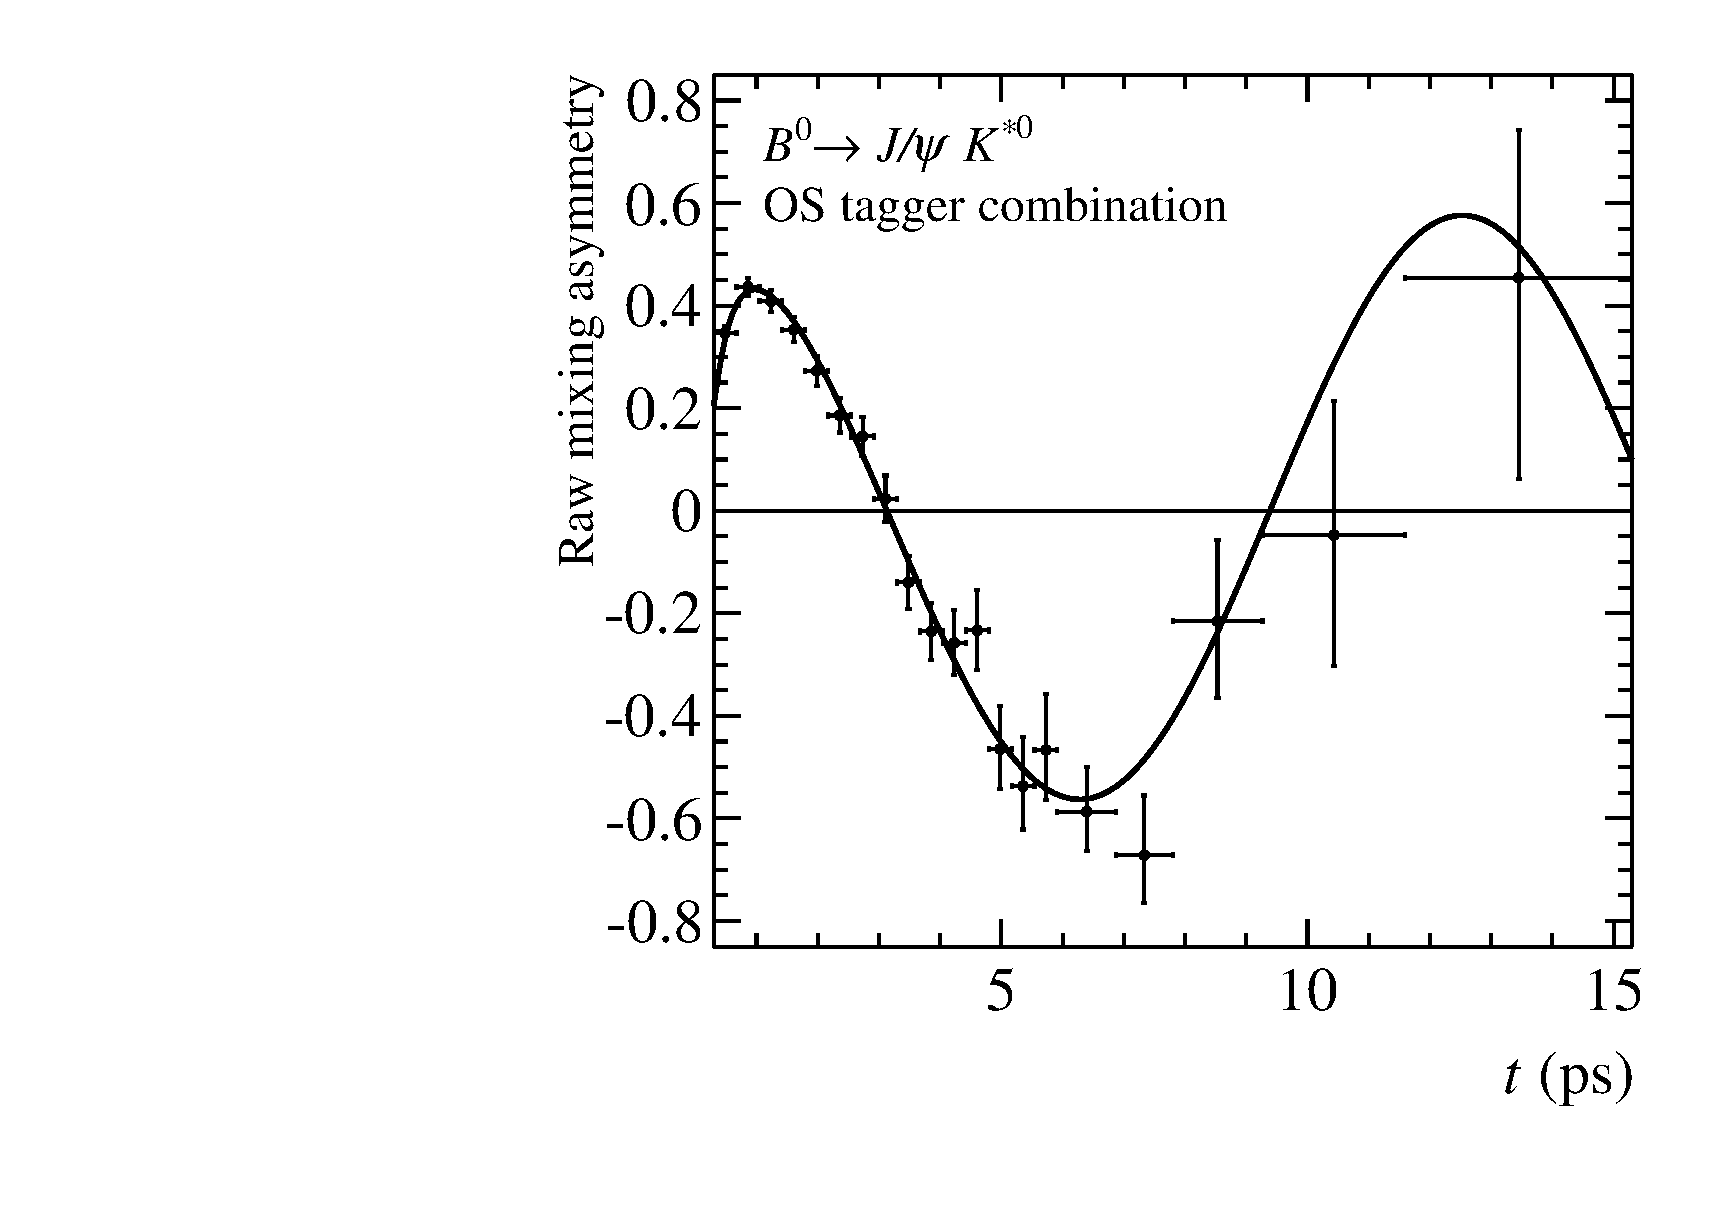
\includegraphics[width=0.4\textwidth, angle=0]{figs/KstAsym.pdf}
		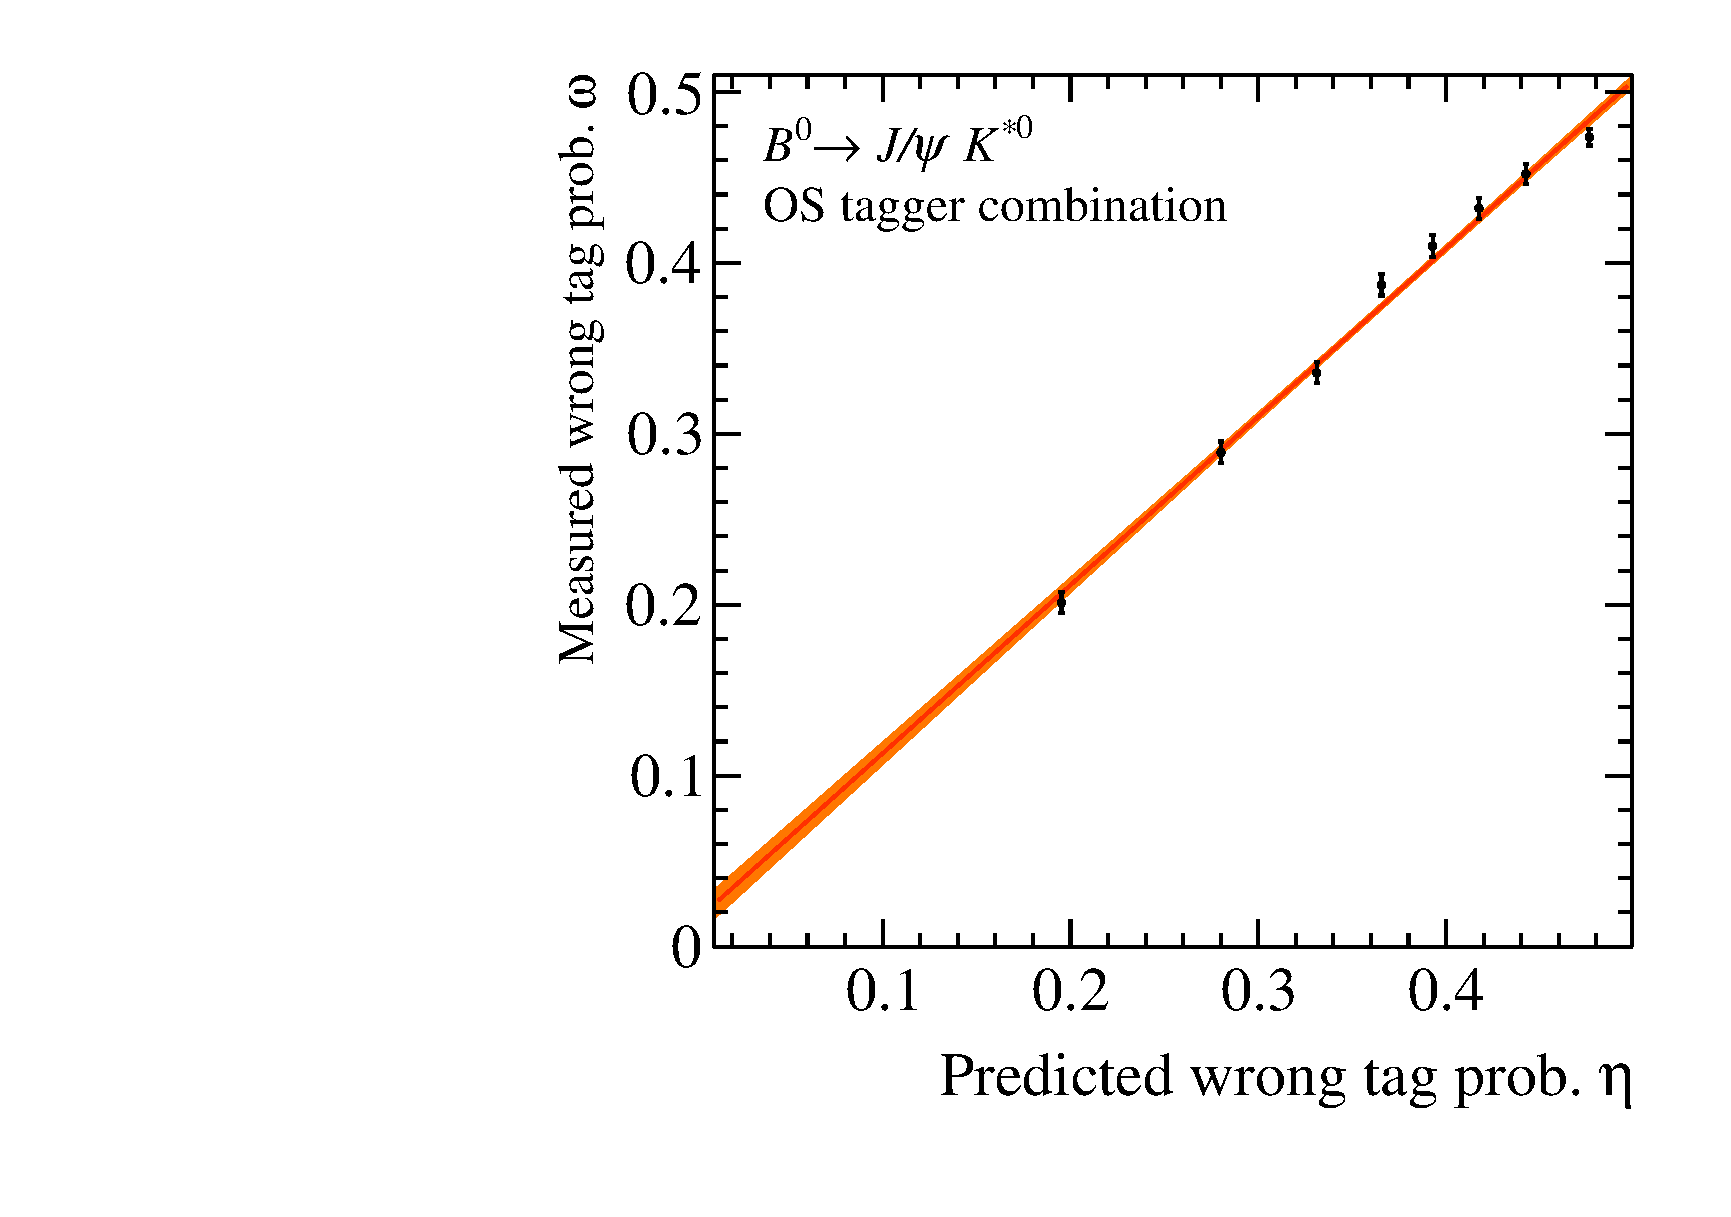
\includegraphics[width=0.4\textwidth, angle=0]{figs/Bd2JpsiKst-Kst-OST-8ScalingFunction_raw.pdf}
		\caption{Mixing asymmetry (left) and calibration function (right) for the OS tagger combination in the calibration mode $B^0\to J\!/\!\psi K^{*0}$.}
		\label{fig:calibration}
	\end{center}
\end{figure}


\section{Flavour Tagging in Run I}\label{sec:4}

\section{Developments}\label{sec:5}

\section{Conclusion}\label{sec:6}

\begin{thebibliography}{99}
\bibitem{1}LHCb Collaboration, R.Aaij et. al., {\it Opposite-side flavour tagging of $B$ mesons at the LHCb experiment, Eur.Phys.J.} C72 (2012) 2022
\bibitem{2}LHCb Collaboration, R. Aaij et. al., {\it Optimization and calibration of the same-side kaon \mbox{tagging} algorithm using hadronic $B_s^0$ decays in 2011 data,} LHCb-CONF-2012-033
\bibitem{3}LHCb Collaboration, R. Aaij et. al., {\it Measurement of $C\!P$ violation and the $B_s^0$ meson decay width difference with   $B_s^0\to J\!/\!\psi K^+K^-$ and \mbox{$\bar{B_s^0}\to J\!/\!\psi \pi^+\pi^-$} decays, } Phys.Rev. D87 (2013) 11, 112010
\bibitem{4}LHCb Collaboration, R. Aaij et. al., {\it Precision measurement of $C\!P$ violation in $B_s^0\to J\!/\!\psi K^+K^-$ decays, } Phys.Rev.Lett. 114 (2015) 4, 041801
\bibitem{5} LHCb Collaboration, R. Aaij et. al., {\it Measurement of the $C\!P$-violating phase $\phi_s$ in $\bar{B_s^0}\to J\!/\!\psi \pi^+\pi^-$ decays, } Phys.Lett. B713 (2012) 378-386
\bibitem{6} LHCb Collaboration, R. Aaij et. al., {\it Measurement of the $C\!P$-violating phase $\phi_s$ in $\bar{B_s^0}\to J\!/\!\psi \pi^+\pi^-$ decays, } Phys.Lett. B736 (2014) 186-195
\bibitem{7} LHCb Collaboration, R. Aaij et. al., {\it Measurement of the $C\!P$-violating phase $\phi_s$ in $\bar{B_s^0}\to D_s^+D_s^-$ decays, } Phys.Rev.Lett. 113 (2014) 21, 211801
\bibitem{8} LHCb Collaboration, R. Aaij et. al., {\it Measurement of $C\!P$ asymmetry in \mbox{$B_s^0\to D_s^\mp K^\pm$} decays, } JHEP 1411 (2014) 060
\bibitem{9} LHCb Collaboration, R. Aaij et. al., {\it Measurement of the time-dependent $C\!P$ asymmetry in $B^0\to J\!/\!\psi K_s^0$ decays, } Phys.Lett. B721 (2013) 24-31

\bibitem{10} LHCb Collaboration, R. Aaij et. al., {\it Measurement of $C\!P$ violation in \mbox{$B^0\to J\!/\!\psi K_s^0$} decays, } Phys.Rev.Lett. 115 (2015) 3, 031601
\bibitem{11} LHCb Collaboration, R. Aaij et. al., {\it Measurement of the time-dependent $C\!P$ asymmetries in $B_s^0\to J\!/\!\psi K_s^0$, } JHEP 1506 (2015) 131
\bibitem{12} LHCb Collaboration, R. Aaij et. al., {\it $B$ flavor tagging using reconstructed charm decays at the LHCb experiment, } LHCb-PAPER-2015.027
\bibitem{13} G. A. Krocker, {\it Development and calibration of a same side kaon tagging algorithm and measurement of the $B_s^0-\bar{B_s^0}$ oscillation frequency $\Delta m_s$ at the LHCb experiment, } PhD thesis, Heidelberg U., Sep, 2013, CERN-THESIS-2013-213

\end{thebibliography} 


\end{document}
